\chapter{Hybrid Langmuir--Machine Learning Modelling}

The present project includes a computational modelling workflow for improving fluoride adsorption prediction using a hybrid Langmuir--Machine Learning approach. The purpose of this modelling stage is to combine the interpretability of adsorption science with the predictive capability of data-driven residual correction. The Langmuir model is used as the baseline adsorption model, and machine learning is used to learn the remaining nonlinear error patterns that are not captured by the baseline model.

The modelling work was organized into three completed phases. In Phase 1, a 500-sample design matrix was generated using Latin Hypercube Sampling across ten adsorption-related factors. A physics-based simulation was then used to generate adsorption capacity values. In Phase 2, a multi-factor Langmuir baseline model was fitted to the simulated adsorption response. In Phase 3, residual analysis and feature engineering were carried out to prepare machine-learning-ready training and testing datasets. This chapter presents the modelling data, algorithmic workflow, residual analysis, and machine learning readiness obtained from the project files.

\section{Computational Modelling Workflow}

The hybrid modelling approach follows a sequential workflow. First, the adsorption factor space is sampled to generate a broad set of operating conditions. Then, fluoride adsorption capacity is estimated using a physics-based response model. The Langmuir baseline model is fitted to this dataset and evaluated using standard regression metrics. The residuals from this model are then analyzed to identify systematic patterns. Finally, engineered features are generated so that machine learning models can learn the residual correction.

\begin{table}[H]
	\centering
	\caption{Hybrid modelling workflow followed in the project}
	\label{tab:hybrid_workflow}
	\renewcommand{\arraystretch}{1.25}
	\resizebox{\textwidth}{!}{
		\begin{tabular}{|c|l|l|l|}
			\hline
			\textbf{Phase} & \textbf{Task} & \textbf{Main Input} & \textbf{Main Output} \\
			\hline
			1 & LHS experimental design & Ten selected adsorption factors & 500 design points \\
			\hline
			1 & Physics-based response simulation & LHS design matrix & Simulated \texttt{q\_removal} dataset \\
			\hline
			2 & Langmuir baseline fitting & Simulated adsorption dataset & Predicted values and residuals \\
			\hline
			3 & Residual analysis & Langmuir residuals & Dominant residual patterns \\
			\hline
			3 & Feature engineering & Original factors and residuals & ML training and testing datasets \\
			\hline
		\end{tabular}
	}
\end{table}

The final hybrid prediction is intended to be calculated by adding the machine-learning residual correction to the Langmuir prediction, as shown below:

\begin{equation}
	q_{hybrid} = q_{Langmuir} + \hat{e}_{ML}
	\label{eq:hybrid_model}
\end{equation}

where $q_{hybrid}$ is the final predicted adsorption capacity, $q_{Langmuir}$ is the baseline Langmuir prediction, and $\hat{e}_{ML}$ is the residual correction predicted by the machine learning model.

\section{Dataset and Input Factor Space}

The modelling dataset was generated using Latin Hypercube Sampling (LHS), which provides uniform coverage of the selected factor space. A total of 500 samples were generated across ten input factors. The factors include major adsorption parameters such as pH, initial fluoride concentration, contact time, adsorbent dose, temperature, and additional water-quality factors such as chloride, hardness, carbonate, and natural organic matter.

\subsection{Experimental Factors and Their Significance}

The selection and scientific justification for each of the ten factors are outlined below:
\begin{itemize}
	\item \textbf{pH (3.01--8.99):} The most critical factor; it controls the surface charge of the adsorbent and fluoride speciation. Optimal removal occurs around pH 6.5.
	\item \textbf{Initial Fluoride Concentration (1.01--9.98 mg/L):} Drives the Langmuir equilibrium and represents typical groundwater contamination levels.
	\item \textbf{Contact Time (10--120 min):} Governs the pseudo-second-order kinetics required to reach adsorption equilibrium.
	\item \textbf{Adsorbent Dose (0.51--5.00 g/L):} Determines the total availability of active adsorption sites.
	\item \textbf{Temperature (20.0--40.0 $^\circ$C):} Influences the adsorption capacity through Arrhenius temperature-dependent kinetics.
	\item \textbf{Flow Rate (0.50--2.00 L/min):} Determines the hydraulic residence time in continuous treatment systems.
	\item \textbf{Chloride (0--100 mg/L):} Acts as a competing anion in the water matrix.
	\item \textbf{Hardness (1--499 mg/L as CaCO$_3$):} Represents cation competition (Ca$^{2+}$/Mg$^{2+}$) for available surface sites.
	\item \textbf{Carbonate (0--100 mg/L as HCO$_3^-$):} A strong competing anion whose effect is highly dependent on pH speciation.
	\item \textbf{Natural Organic Matter (0--50 mg/L):} Causes pore fouling, which physically blocks access to the adsorbent's internal surface area.
\end{itemize}

\begin{table}[H]
	\centering
	\caption{Input factors used for the computational modelling dataset}
	\label{tab:modelling_factors}
	\renewcommand{\arraystretch}{1.2}
	\resizebox{\textwidth}{!}{
		\begin{tabular}{|c|l|c|c|l|}
			\hline
			\textbf{Sl. No.} & \textbf{Factor} & \textbf{Minimum} & \textbf{Maximum} & \textbf{Unit} \\
			\hline
			1 & pH & 3.01 & 8.99 & -- \\
			\hline
			2 & Initial fluoride concentration, $C_0$ & 1.01 & 9.98 & mg/L \\
			\hline
			3 & Contact time & 10 & 120 & min \\
			\hline
			4 & Adsorbent dose & 0.51 & 5.00 & g/L \\
			\hline
			5 & Temperature & 20.0 & 40.0 & $^\circ$C \\
			\hline
			6 & Flow rate & 0.502 & 1.999 & L/min \\
			\hline
			7 & Chloride concentration & 0 & 100 & mg/L \\
			\hline
			8 & Hardness & 1 & 499 & mg/L as CaCO$_3$ \\
			\hline
			9 & Carbonate concentration & 0 & 100 & mg/L as HCO$_3^-$ \\
			\hline
			10 & Natural organic matter & 0 & 50 & mg/L \\
			\hline
		\end{tabular}
	}
\end{table}

The generated dataset contains 500 rows and 13 columns, including run number, input factors, randomization order, and adsorption response. The simulated adsorption capacity \texttt{q\_removal} varied from 1.4166 mg/g to 8.3156 mg/g, with a mean value of 4.0989 mg/g and a standard deviation of 1.2309 mg/g. These values indicate a physically reasonable adsorption capacity range for the modelling study.

\begin{table}[H]
	\centering
	\caption{Summary of generated adsorption response data}
	\label{tab:response_summary}
	\renewcommand{\arraystretch}{1.2}
	\begin{tabular}{|l|c|}
		\hline
		\textbf{Quantity} & \textbf{Value} \\
		\hline
		Total samples & 500 \\
		\hline
		Number of input factors & 10 \\
		\hline
		Minimum \texttt{q\_removal} & 1.4166 mg/g \\
		\hline
		Maximum \texttt{q\_removal} & 8.3156 mg/g \\
		\hline
		Mean \texttt{q\_removal} & 4.0989 mg/g \\
		\hline
		Standard deviation & 1.2309 mg/g \\
		\hline
	\end{tabular}
\end{table}

\section{Physics-Based Response Generation}

The response generation script was developed to simulate fluoride adsorption capacity under different operating conditions. The simulation considered important adsorption mechanisms such as pH-dependent adsorption, concentration effect, contact-time response, temperature effect, dose saturation, flow-rate effect, ion competition, and natural organic matter fouling. The reference Langmuir parameters used in the simulation were $q_{max}=8.5$ mg/g and $K_L=0.12$ L/mg at 25 $^\circ$C. The optimum pH was taken as 6.5, and a bell-curve relationship was used to represent pH-dependent adsorption behaviour.

The pH effect was modelled using:

\begin{equation}
	f_{pH} = \exp \left[-\frac{(pH - 6.5)^2}{2(1.1)^2}\right]
	\label{eq:ph_effect}
\end{equation}

This relationship gives maximum adsorption near pH 6.5 and lower adsorption at strongly acidic or alkaline conditions. Ion competition and natural organic matter effects were included as moderate reduction factors so that the simulated response remained physically realistic. A small measurement noise of 5\% was also added to represent experimental variability.

\section{Langmuir Baseline Model}

The Phase 2 model used the simulated adsorption dataset to fit a multi-factor Langmuir baseline model. The ten original factors were standardized and expanded into second-order polynomial features. This produced 66 model features, including original terms, squared terms, and two-way interaction terms. A linear regression model was then fitted on the expanded feature matrix to estimate adsorption capacity.

The residual error was calculated as:

\begin{equation}
	e = q_{actual} - q_{predicted}
	\label{eq:residual}
\end{equation}

where $q_{actual}$ is the simulated adsorption capacity and $q_{predicted}$ is the Langmuir baseline prediction.

\begin{table}[H]
	\centering
	\caption{Performance of the Langmuir baseline model}
	\label{tab:langmuir_performance}
	\renewcommand{\arraystretch}{1.2}
	\begin{tabular}{|l|c|}
		\hline
		\textbf{Metric} & \textbf{Value} \\
		\hline
		Number of samples & 500 \\
		\hline
		Original factors & 10 \\
		\hline
		Expanded polynomial features & 66 \\
		\hline
		Model type & Multi-factor Langmuir polynomial model \\
		\hline
		$R^2$ & 0.8158 \\
		\hline
		RMSE & 0.5278 mg/g \\
		\hline
		MAE & 0.4282 mg/g \\
		\hline
		Residual mean & $-6.63 \times 10^{-16}$ \\
		\hline
		Residual standard deviation & 0.5278 mg/g \\
		\hline
	\end{tabular}
\end{table}

The Langmuir baseline model explained 81.58\% of the variation in adsorption capacity. The near-zero residual mean indicates that the model was unbiased overall. However, the remaining residual variation showed systematic behaviour, which supports the use of machine learning for residual correction.

\begin{figure}[H]
	\centering
	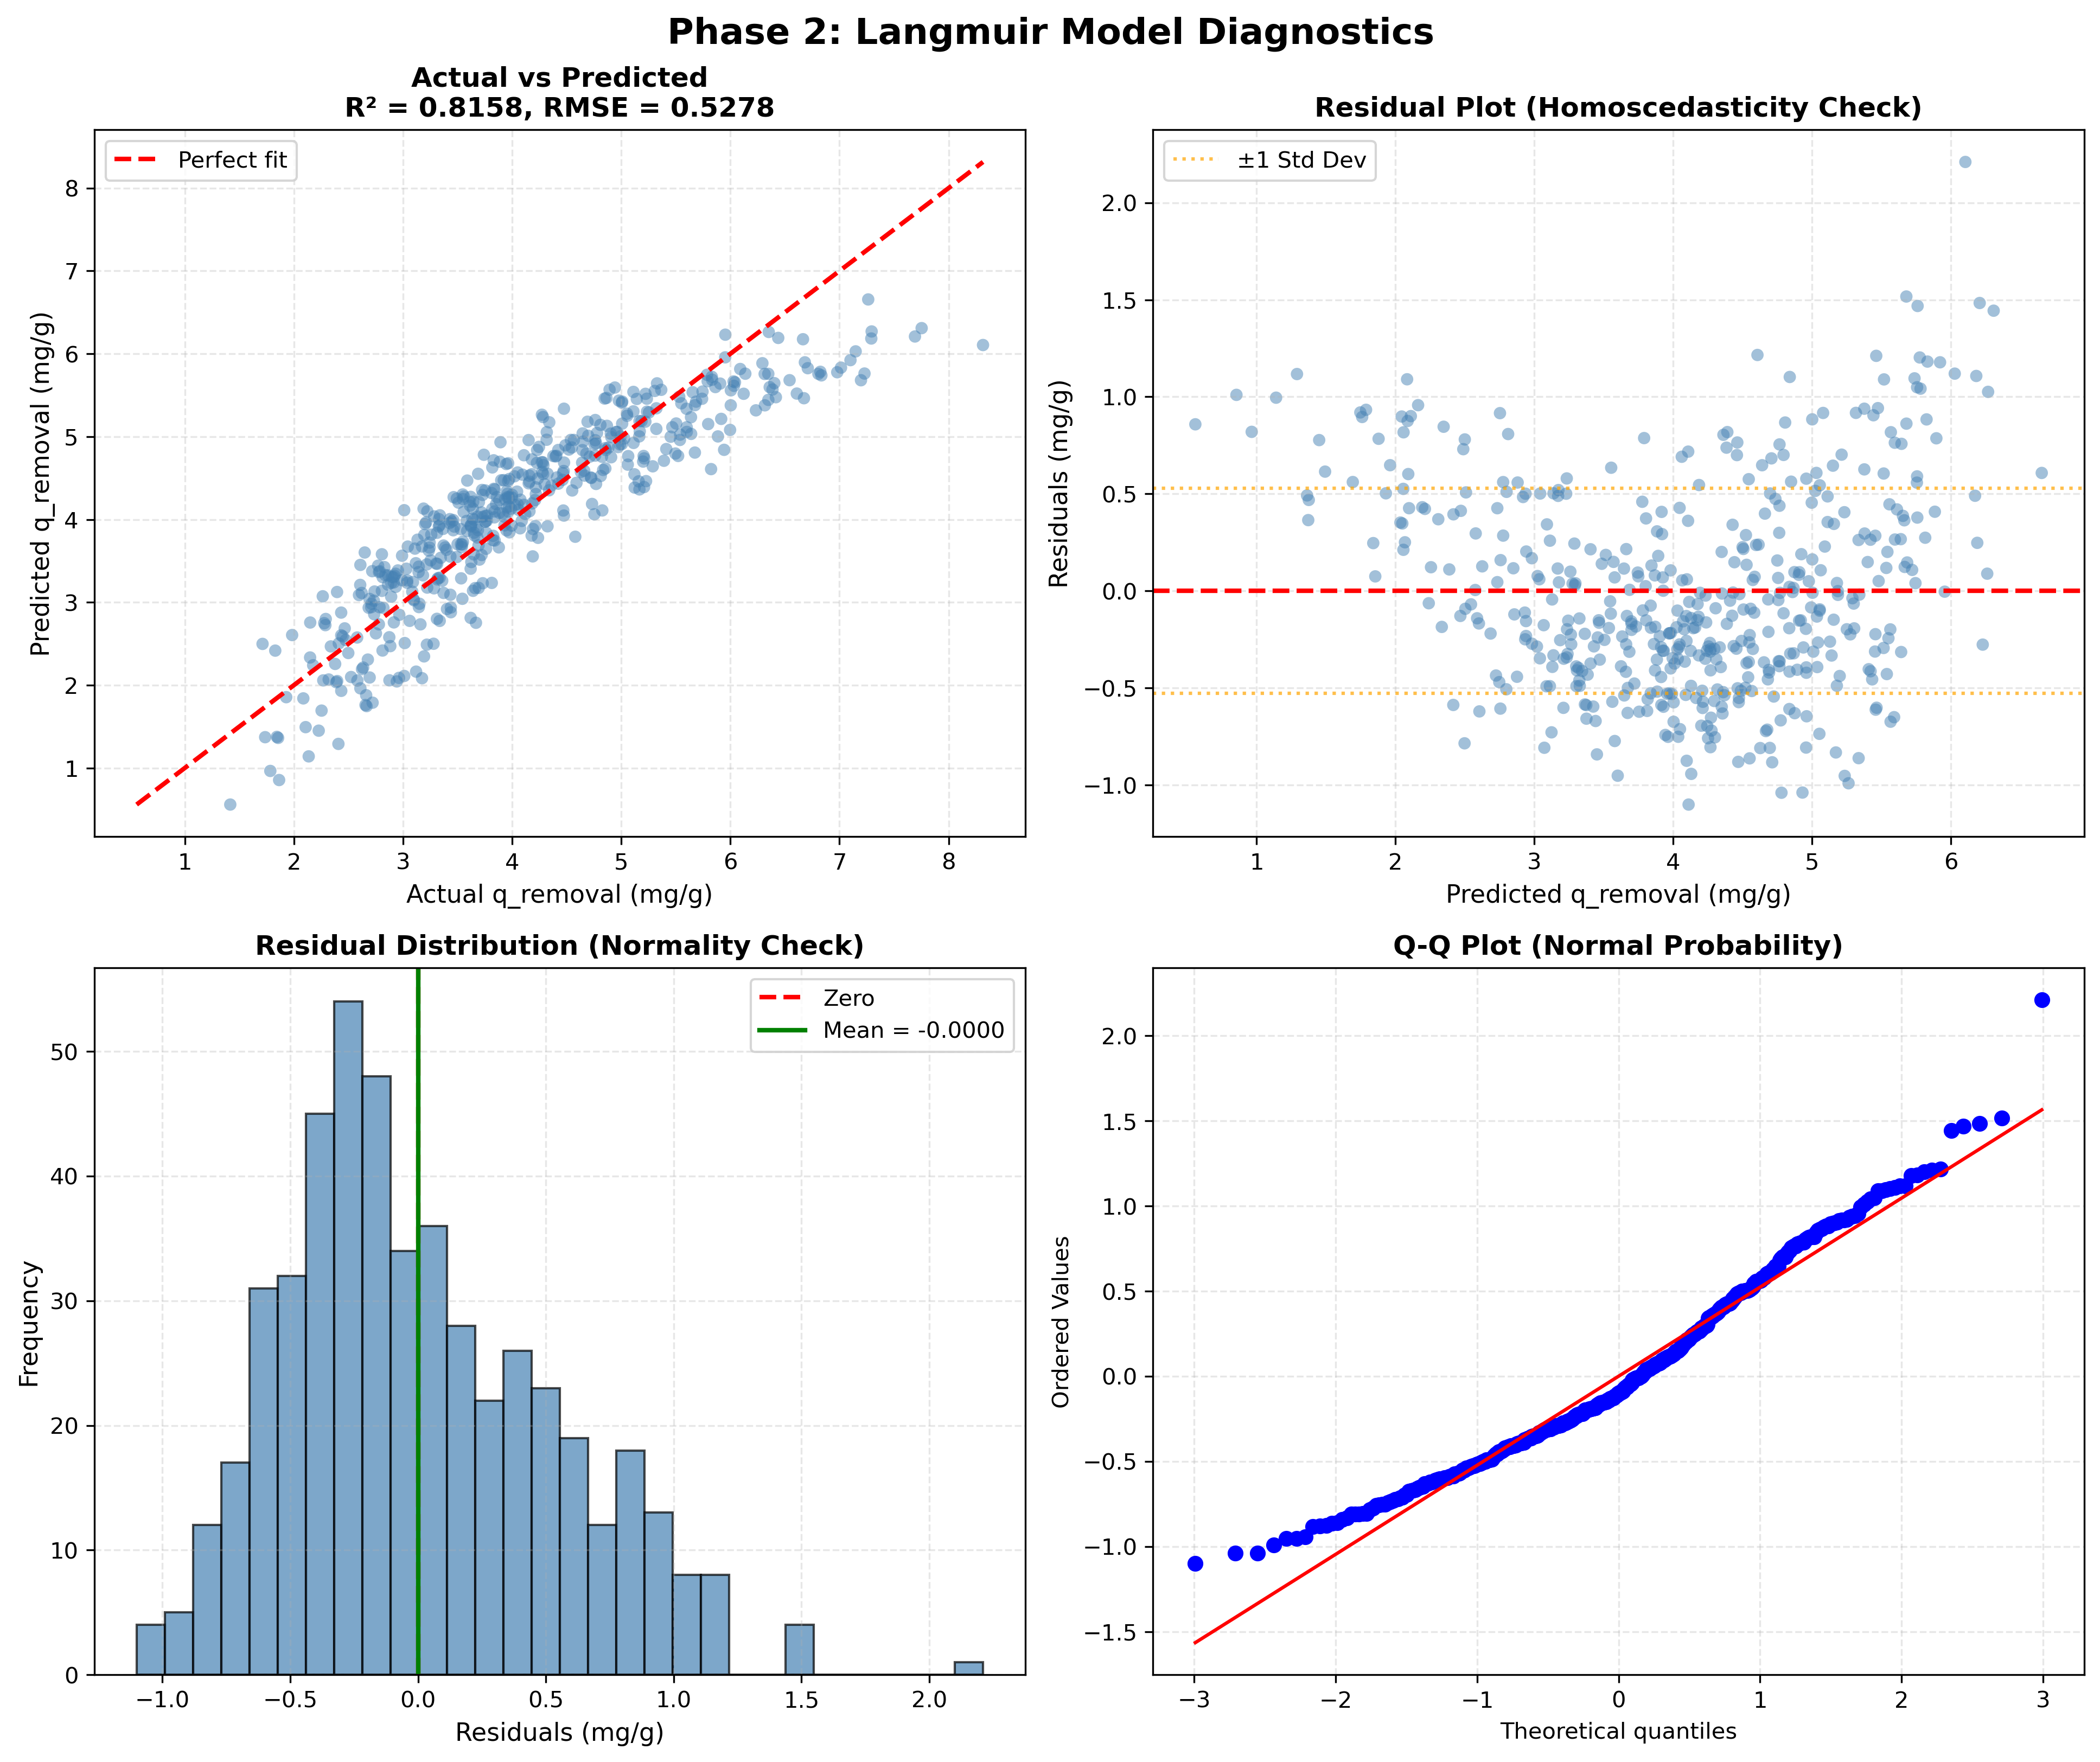
\includegraphics[width=0.85\textwidth]{Chapter5/Figures/langmuir_diagnostics.png}
	\caption{Diagnostic plots obtained from the Langmuir baseline model}
	\label{fig:langmuir_diagnostics_ch5}
\end{figure}

\section{Residual Analysis}

Residual analysis was carried out to identify the patterns not captured by the Langmuir baseline model. The residuals ranged from -1.1008 mg/g to 2.2100 mg/g. The strongest pattern was observed with pH. The model underestimated adsorption near the optimum pH range and overestimated adsorption in some acidic regions. This indicates that the polynomial approximation could not completely capture the bell-shaped pH behaviour introduced during response generation.

\begin{table}[H]
	\centering
	\caption{pH-wise residual pattern observed after Langmuir fitting}
	\label{tab:ph_residual_pattern}
	\renewcommand{\arraystretch}{1.2}
	\resizebox{\textwidth}{!}{
		\begin{tabular}{|l|c|c|c|}
		\hline
		\textbf{pH range} & \textbf{Number of points} & \textbf{Mean residual (mg/g)} & \textbf{Interpretation} \\
		\hline
		pH 3--4 & 84 & 0.2478 & Underestimation \\
		\hline
		pH 4--5 & 83 & -0.5250 & Overestimation \\
		\hline
		pH 5--6 & 84 & -0.1172 & Mild overestimation \\
		\hline
		pH 6--6.5 & 41 & 0.4706 & Underestimation \\
		\hline
		pH 6.5--7 & 42 & 0.6491 & Strong underestimation \\
		\hline
		pH 7--7.5 & 41 & 0.2082 & Underestimation \\
		\hline
		pH 7.5--8 & 42 & -0.1760 & Overestimation \\
		\hline
		pH 8--9 & 83 & -0.1819 & Overestimation \\
		\hline
		\end{tabular}
	}
\end{table}

The most important residual finding was observed in the pH 6.5--7 range, where the mean residual was +0.6491 mg/g. A positive residual means that the baseline model predicted a lower adsorption value than the actual response. Therefore, this region provides an important opportunity for machine learning correction.

\begin{figure}[H]
	\centering
	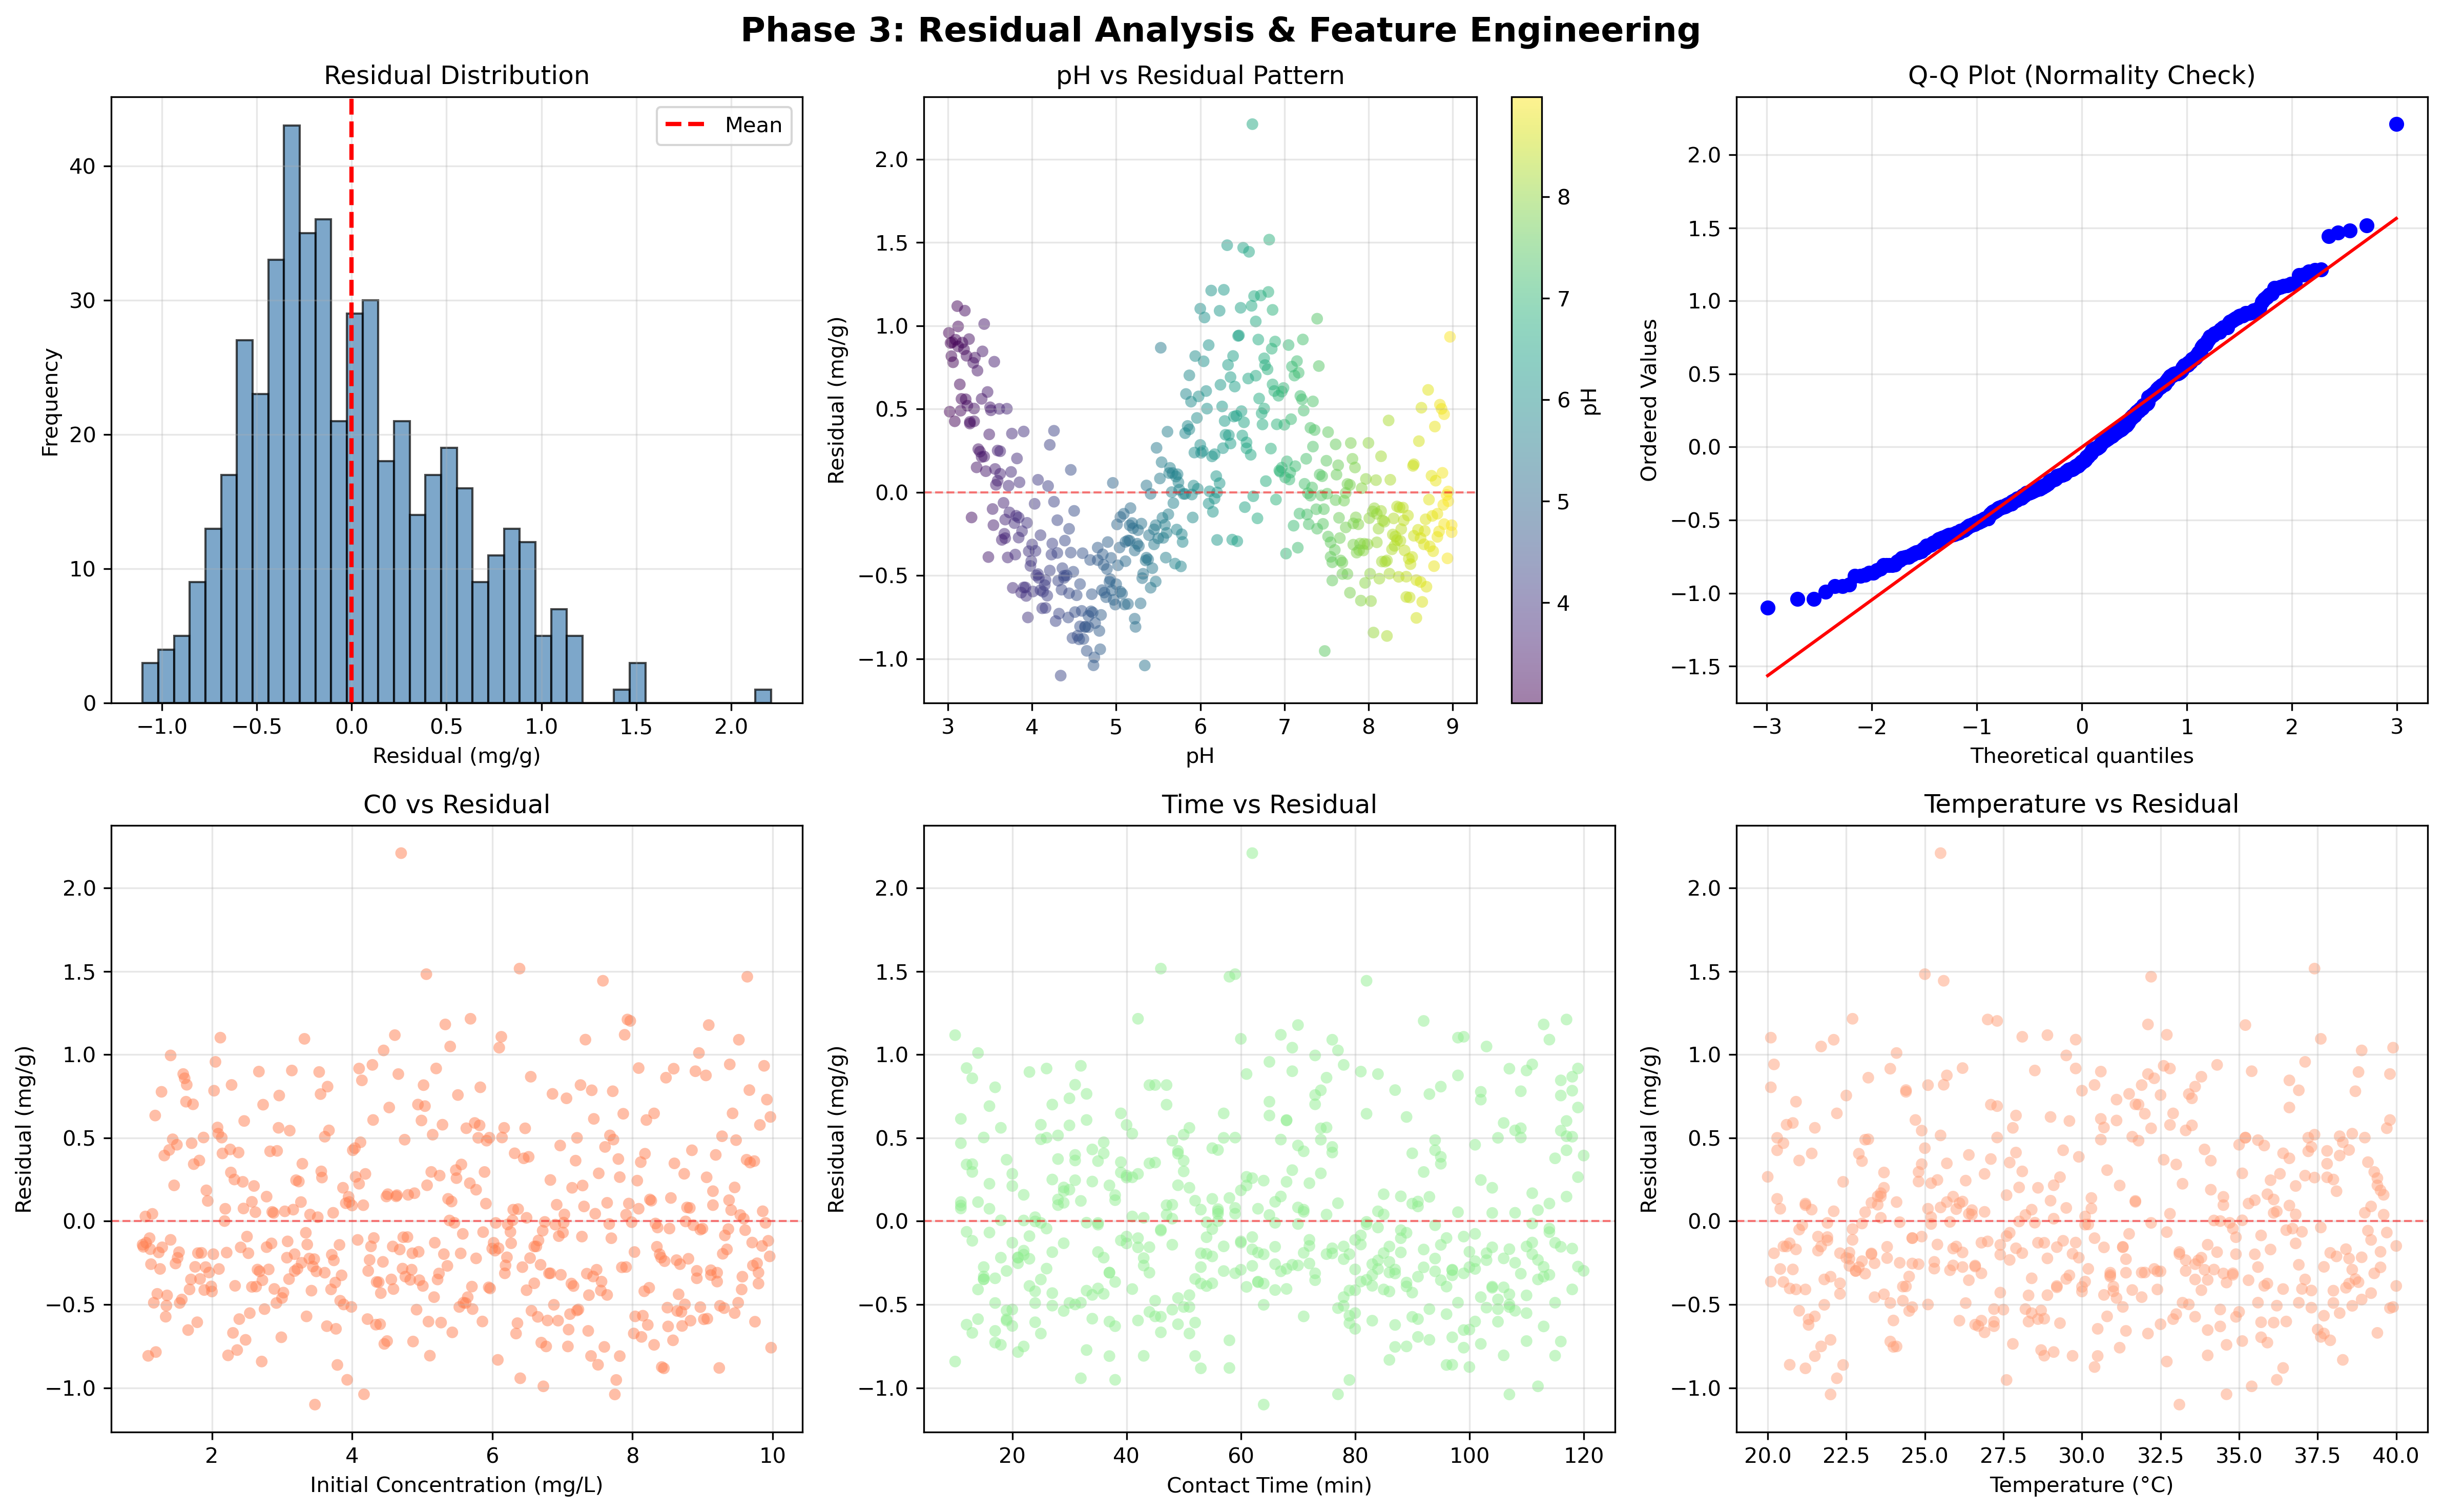
\includegraphics[width=0.9\textwidth]{Chapter5/Figures/phase3_diagnostics.png}
	\caption{Residual analysis and feature engineering diagnostic plots}
	\label{fig:phase3_diagnostics_ch5}
\end{figure}

\section{Feature Engineering for Machine Learning}

Feature engineering was carried out to convert the original factor data into more informative machine learning inputs. The original ten factors were retained, and 28 new features were generated. Therefore, the final feature matrix contained 38 input features. The engineered features were grouped into pH-deviation features, ion-competition features, equilibrium and loading features, logarithmic transformations, interaction terms, and composite performance indicators.

\begin{table}[H]
	\centering
	\caption{Feature engineering groups used for residual learning}
	\label{tab:feature_engineering_groups}
	\renewcommand{\arraystretch}{1.2}
	\resizebox{\textwidth}{!}{
		\begin{tabular}{|l|c|l|}
			\hline
			\textbf{Feature group} & \textbf{Number of features} & \textbf{Purpose} \\
			\hline
			Original adsorption factors & 10 & Preserve direct experimental variables \\
			\hline
			pH deviation features & 5 & Capture distance from optimum pH 6.5 \\
			\hline
			Ion competition features & 5 & Represent combined effects of chloride, hardness, and carbonate \\
			\hline
			Equilibrium and loading features & 5 & Represent dose, concentration, time, and fouling effects \\
			\hline
			Logarithmic transforms & 5 & Capture nonlinear scale effects \\
			\hline
			Interaction terms & 5 & Represent coupled factor effects \\
			\hline
			Composite indicators & 3 & Represent combined performance and stress conditions \\
			\hline
			Total input features & 38 & Machine learning feature matrix \\
			\hline
		\end{tabular}
	}
\end{table}

The final dataset was divided into training and testing subsets. The training dataset contained 400 samples, and the testing dataset contained 100 samples. Both datasets contained 38 input features and one residual target column. This prepared dataset is suitable for training residual correction models such as Random Forest, XGBoost, and Multi-Layer Perceptron.

\section{Feature Importance and ML Readiness}

A quick Random Forest model was trained during Phase 3 to verify whether the residual pattern was learnable. The model achieved a training $R^2$ of 0.9039 and a testing $R^2$ of 0.4729 on residual prediction. This result shows that the residuals are not random and contain learnable structure. The feature importance ranking also confirmed that pH-related features dominate the residual correction problem.

\begin{table}[H]
	\centering
	\caption{Top feature importance values from quick Random Forest residual model}
	\label{tab:feature_importance}
	\renewcommand{\arraystretch}{1.2}
	\begin{tabular}{|c|l|c|}
		\hline
		\textbf{Rank} & \textbf{Feature} & \textbf{Importance} \\
		\hline
		1 & \texttt{pH\_abs\_dev} & 0.2109 \\
		\hline
		2 & \texttt{pH\_dev\_sq} & 0.1669 \\
		\hline
		3 & \texttt{performance\_index} & 0.0787 \\
		\hline
		4 & \texttt{optimal\_pH\_score} & 0.0523 \\
		\hline
		5 & \texttt{pH} & 0.0498 \\
		\hline
		6 & \texttt{pH\_dev} & 0.0478 \\
		\hline
		7 & \texttt{pH\_optimal} & 0.0454 \\
		\hline
		8 & \texttt{pH\_gaussian} & 0.0440 \\
		\hline
	\end{tabular}
\end{table}

The top two features, \texttt{pH\_abs\_dev} and \texttt{pH\_dev\_sq}, together contributed strongly to residual prediction. This confirms that the baseline Langmuir polynomial model captured the broad adsorption behaviour but did not fully represent the nonlinear pH optimum. The prepared Phase 3 outputs therefore provide the required foundation for Phase 4 machine learning model training and Phase 5 hybrid model integration.

This chapter presented the complete modelling information extracted from the project files, including dataset generation, Langmuir baseline fitting, residual analysis, feature engineering, and machine learning readiness. The experimental results, biomaterial preparation observations, CCD adsorption runs, and Langmuir diagnostic outcomes are discussed in the next chapter.
